\documentclass[a4paper,10pt]{article}

\usepackage[utf8]{inputenc}
%\usepackage[T1]{fontenc}

\usepackage{textcomp}           % Extra Symbole (Grad Celsius etc.)
\usepackage{amssymb,amsmath}    % Schöne Formeln (AMS = American Mathematical Society)
\usepackage{graphicx}           % Bilder und Seitenränder
\usepackage{subcaption}			% captions for subfigures
\usepackage{booktabs}           % Schönere Tabellen
\usepackage{colortbl}           % Farbige Tabellen

%\usepackage{tcolorbox}			% schöne bunte Boxen
\usepackage{mathtools}			% \mathclap für ordentliche \underbrace-			environments
\usepackage[left=2cm,right=2cm,top=2cm,bottom=2cm]{geometry}			% Pagelayout mit \newgeometry, \restoregeometry
\usepackage{float}
\usepackage{wrapfig}
\usepackage{enumitem}
\usepackage{float}
\usepackage{braket}
\usepackage{caption}
\usepackage[per-mode=reciprocal,output-decimal-marker={.},binary-units=true,separate-uncertainty=true]{siunitx}
\usepackage[breaklinks=true,colorlinks=true,linkcolor=blue,urlcolor=blue,citecolor=blue]{hyperref}
\usepackage{physics}
\usepackage{url}
\usepackage{subcaption}
\usepackage{calrsfs}
\DeclareMathAlphabet{\pazocal}{OMS}{zplm}{m}{n}
\usepackage{tikz}
\usetikzlibrary{decorations, positioning, intersections, calc, shapes,arrows, scopes}
\usepackage{pgfplots}
\usepackage{bodegraph}
\usepackage{circuitikz}
\usepackage{chemfig}
\usepackage{chemformula}
\usepackage[toc,page]{appendix}
\graphicspath{{./img/}}
\usepackage{verbatim}

\DeclareSIUnit\elementarycharge{e}

\newcommand{\dif}{\mathrm{d}}

\bibliographystyle{unsrtnat}

\renewcommand{\k}{\mathbf{k}}
\begin{document}
\begin{titlepage}
 \begin{center}
	\Large{Advanced laboratory course 3}
	\end{center}
	\begin{center}
	 \LARGE{\textbf{FP3 - Rare gas clusters}}
	\end{center}

	\begin{center}

	\large Marco \textsc{Canteri} \\
	marco.canteri@student.uibk.ac.at\\
	\large Maximilian Gerold \textsc{Münst} \\
	maximilian.muenst@student.uibk.ac.at
	\end{center}

	\begin{center}
	\vspace{1cm}
	Innsbruck, \today
	\vspace{1cm}
	\end{center}

	\begin{abstract}
	We created neon clusters via superbeam expansion technique, we then studied the isotope population of the clusters, magic numbers, and energy appearance. Moreover, we studied the
	impact of air as pick-up gas in the neon clusters.
    \end{abstract}
    \vspace{1cm}

	\begin{center}
	
\includegraphics[scale=0.56]{img/uibk}
	\end{center}

\end{titlepage}


\section{Introduction}
In this experiment we explored the world of clusters, which are an aggregate of atoms with no particular structure. Cluster are the missing link between molecules and condensed matter, their wide applications are fundamental in nanotechnology, where clusters are the building blocks of the technology.

\section{Theoretical Background}
In this experiment one produces Neon clusters by expanding Neon gas. According to \cite{script}, Neon has an average mass of \SI{20.18}{\atomicmassunit}, with an isotope abundance of \ch{^{20}Ne}: $90.92\%$, \ch{^{21}Ne}: $0.26\%$ and \ch{^{22}Ne}: $8.82\%$.
%What's neon? And what's the meaning of a neon cluster? Can we reach god with it? Can we finally understand the meaning of life?\\
%These and more questions will be answered in this section. You will be surprised that the answer is $42$.

\subsection{Gas expansion}
There are different ways to produce clusters, however, usually those methods are built on 4 steps:
\begin{itemize}
	\item Vaporization (producing sufficiently cold particles in the gas phase)
	\item Nucleation (Condensation of gaseous atoms to form a cluster nucleus)
	\item Growth (adding particles to existing nuclei)
	\item Coalescence (Merging of small clusters)
\end{itemize}
To start the formation of clusters the thermal energy has to be smaller than the binding energy of the cluster. To achieve sufficiently low temperatures, the gas is first stored at a low temperature while being at a very high pressure. The gas can escape from this high pressure environment via a nozzle into a vacuum chamber. The rapid expansion changes the velocity distribution from a Maxwell-Boltzmann distribution to a floating Maxwellian distribution, meaning that the distribution gets narrower and more symmetrical around the mean velocity. \\
As one is dealing with adiabatic expansion the enthalpy is conserved, meaning that one can write
\begin{equation}
	c_\mathrm{p} T_0 = c_\mathrm{p} T + \frac{m u^2}{2},
\end{equation}
where $c_\mathrm{p}$ is the heat capacity at constant pressure, $m$ is the mass of the atom, $u$ is the drift velocity of the gas and $T$ and $T_0$ are the temperatures at and before expansion. From here it is possible to derive a set of equations.
\begin{equation}
	\begin{split}
	T &= T_0 \left[1 + \frac{\gamma - 1}{2} M^2 \right]^{-1} \\
	p &= p_0 \left[1 + \frac{\gamma - 1}{2} M^2 \right]^{\frac{1}{1 - \gamma}} \\
	\rho &= \rho_0 \left[1 + \frac{\gamma - 1}{2} M^2 \right]^{\frac{\gamma}{1-\gamma}} \\
	\end{split}
\end{equation}
Here, $\gamma$ represents the adiabatic exponent and $M = u/v_s$ is the Mach number. As one can imagine, all these parameters decrease steeply during the expansion.

\subsection{Cluster formation}
To generate a dimer, i.e. a two atom cluster, a three body collision is necessary in order to conserve energy and momentum.
\begin{equation}
	\ch{A} + \ch{A} + \ch{A} \rightarrow \ch{2 A} + \ch{A}
\end{equation}
As the cluster grows condensation heat builds up in the cluster and can only be emitted by release of a monomer, i.e. a single atom. \\
Growth can be described by classical fluid-gas phase transitions. The vapour pressure line divides said states as is shown in Fig. \ref{fig_formation}. However growth only occurs once supersaturation appears. This is due to surface tension of the cluster. According to \cite{script} the critical radius for cluster growth is
\begin{equation}
	r^\ast = \frac{2 \sigma m}{k_\mathrm{B} T \rho} \frac{1}{\ln(\phi_\mathrm{k})},
\end{equation}
where $\sigma$ describes the surface tension, $T$ the temperature, $\rho$ the density and $\phi_\mathrm{k} = p_\mathrm{k} / p_\infty$ is the supersaturation condition. Clusters above their critical radius will accumulate more atoms, while those below evaporate monomers until the condition is fulfilled.
\begin{figure}
	\centering
	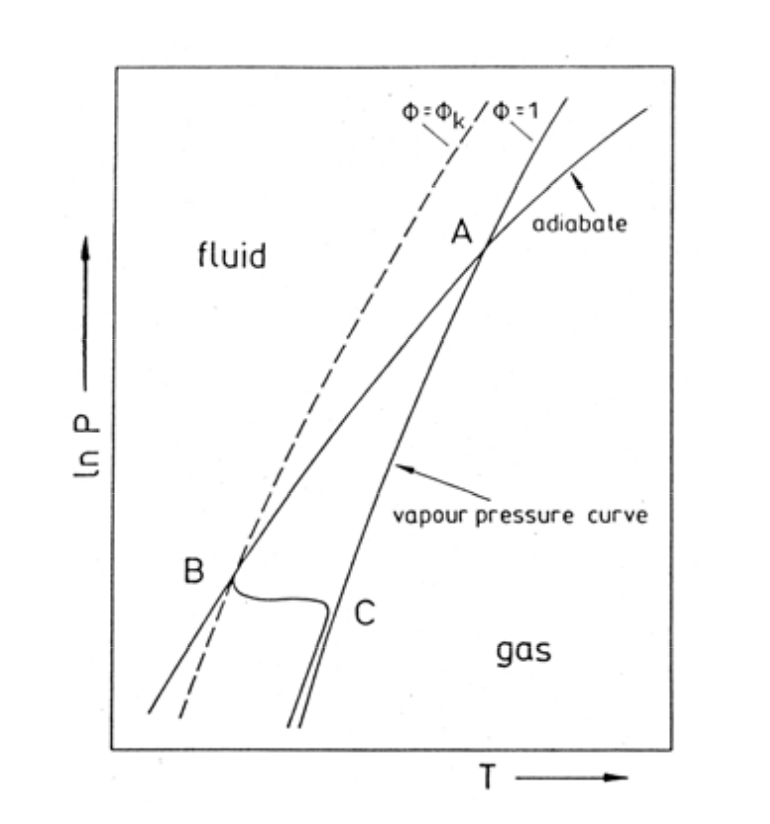
\includegraphics[width = 0.5 \textwidth]{formation.png}
	\caption{Phase diagram containing a growth line of a cluster. The image was taken from \cite{script}. }
	\label{fig_formation}
\end{figure}
Fig. \ref{fig_formation} shows the growth of a cluster. The cluster state follows an adiabatic line from the gaseous into the fluid state. But only when the supersaturation condition is fulfilled, the cluster acquires an additional component. The release of the condensation heat brings the cluster back to the equilibrium between liquid and gaseous state. \\
Empirically, the mean cluster size is determined as
\begin{equation}
	\bar{N} = \frac{p_0 D^{1.5}}{T_0^{2.4}}.
\end{equation}
Again, $T_0$ and $p_0$ describe the temperature and pressure in the stagnation chamber. $D = d / \tan \theta$ represents the reduced diameter of the nozzle, where $\theta$ is half the opening angle of the nozzle. As one can see, reducing the temperature in the stagnation chamber has the highest impact on the mean size of the clusters.

\section{Experimental Setup}
Basically, the setup in this experiment has to first produce and grow clusters of Neon atoms and in a second step ionize said clusters. Finally the ionized clusters have to be detected.

\subsection{Cluster source}
In this setup cluster nuclei are generated by means of supersonic expansion of the source gas. Neon gas is stored in a stagnation chamber at roughly \SI{13}{\bar} and low temperature. It is then released into a vacuum chamber where the gas adiabatically expands at supersonic speed. It is noteworthy that the gas velocity is approximately constant during the expansion, but the quickly decreasing speed of sound gradually increases the local Mach number. \\
Fig. \ref{fig_expansion} shows a sketch of the expansion cone generated by the Neon gas. As there is a low but finite background pressure in the expansion chamber, two shock zones develop: a barrel shock, which is formed symmetrically around the central axis of the expansion zone and a termination shock at the end of the expansion region, referred to as the Mach disk. Together, these shock fronts shield what is called the zone of silence from the background gas, which means that in the zone of silence there is hardly any collisions with the background gas to be expected. According to \cite{script} the position of the Mach disk can be calculated as
\begin{equation}
	\frac{x_\mathrm{M}}{d} = 0.67 \sqrt{\frac{p_0}{p_\mathrm{b}}},
\end{equation}
where $d$ is the diameter of the nozzle, $p_0$ and $p_\mathrm{b}$ represent the stagnation pressure and the background pressure respectively. In Fig. \ref{fig_expansion} the Mach disk is depicted once for an undistorted case as a dash-dotted line and once as a solid line which is distorted by a skimmer. \\
The skimmer collects only the central component of the gas jet and guides it into the cluster chamber, where the clusters are formed by nucleation. It has to be positioned with care, as if it is placed to close to the nozzle, one will see turbulences in the expansion, while placing it behind the Mach disk results in considerable loss in intensity, as the collisions with the background gas are to be expected. The formed clusters are subsequently collided with an electron beam, such that the neutral clusters are positively ionized via electron ionization. The ions now can be analyzed with a mass spectrometer, for this experiment we used a linear quadrupole mass spectrometer.%\\
%The electron beam is created by evaporation from a filament, the beam is focused with a set of electron lenses and filtered by energy with an hemispherical electron monochromator.

\begin{figure}[htp!]
	\centering
	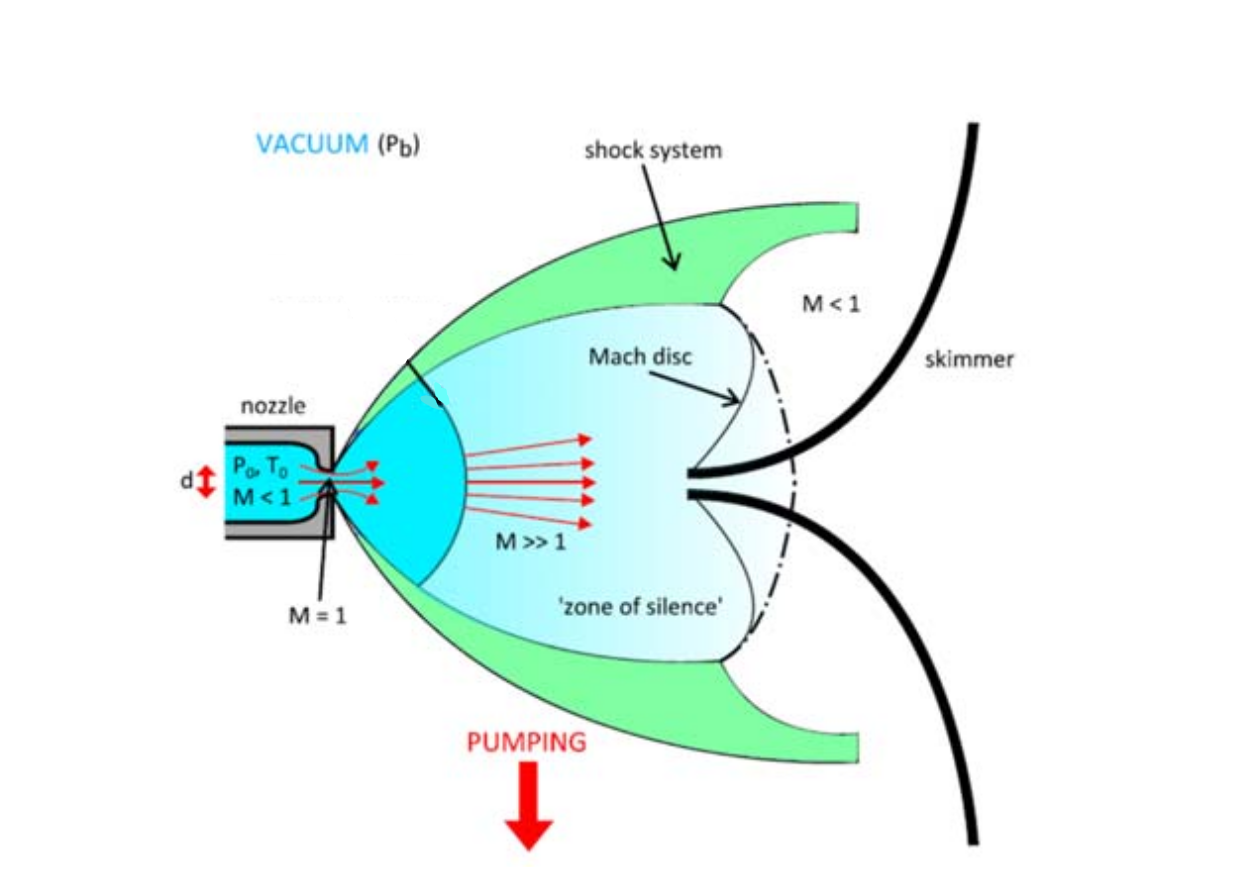
\includegraphics[width = 0.6 \textwidth]{expansion.png}
	\caption{Sketch of the expansion cone of the Neon gas. The figure was taken from \cite{script}. }
	\label{fig_expansion}
\end{figure}

\subsection{Electron monochromator}

As the setup used in this experiment is also used for research, we could not install or set up any components ourselves. All could be done was tune the voltages on several electrostatic lenses.
\\
A hairpin filament serves as electron source in this setup. A current of roughly \SI{2.35}{\ampere} is passed through the filament which leads to an emitted current of several \SI{10}{\micro \ampere}. As these electrons are emitted roughly isotropically in all directions with their kinetic energies following a Boltzmann distribution, a field generated by an anode collects the electrons of the source chamber and guides them into an array of 3-element lenses, which collimate and focus the electron beam. A depiction of the setup is shown in Fig. \ref{setup}.
\\
The focused beam of electrons is then guided towards a hemispherical energy selector. As Fig. \ref{setup} indicates. This component consists of two concentric hemispherical surfaces which are kept at different but constant voltages, which leads to a constant spherically symmetry field in the monochromator. This way an energy filter is created, as electrons which are too fast will collide with the outer surface, while electrons that are too slow will be absorbed by the inner element. Variation of these two voltages allows for a variation of the energy of the electron beam, while the energy resolution is maintained.
\\
The energy filter is followed by a second set of electrostatic lenses, which again collect the flux of electrons after the monochromator and focuses the beam into the collision chamber. Positive ions are created upon impact of an electron onto a cluster. These resulting ions are guided into the quadrupole mass filter, which analyses the charge-mass-ratio. Electrons that to not hit a target are collected in a Faraday cup at the back of the collision chamber.

\begin{figure}[H]
	\centering
	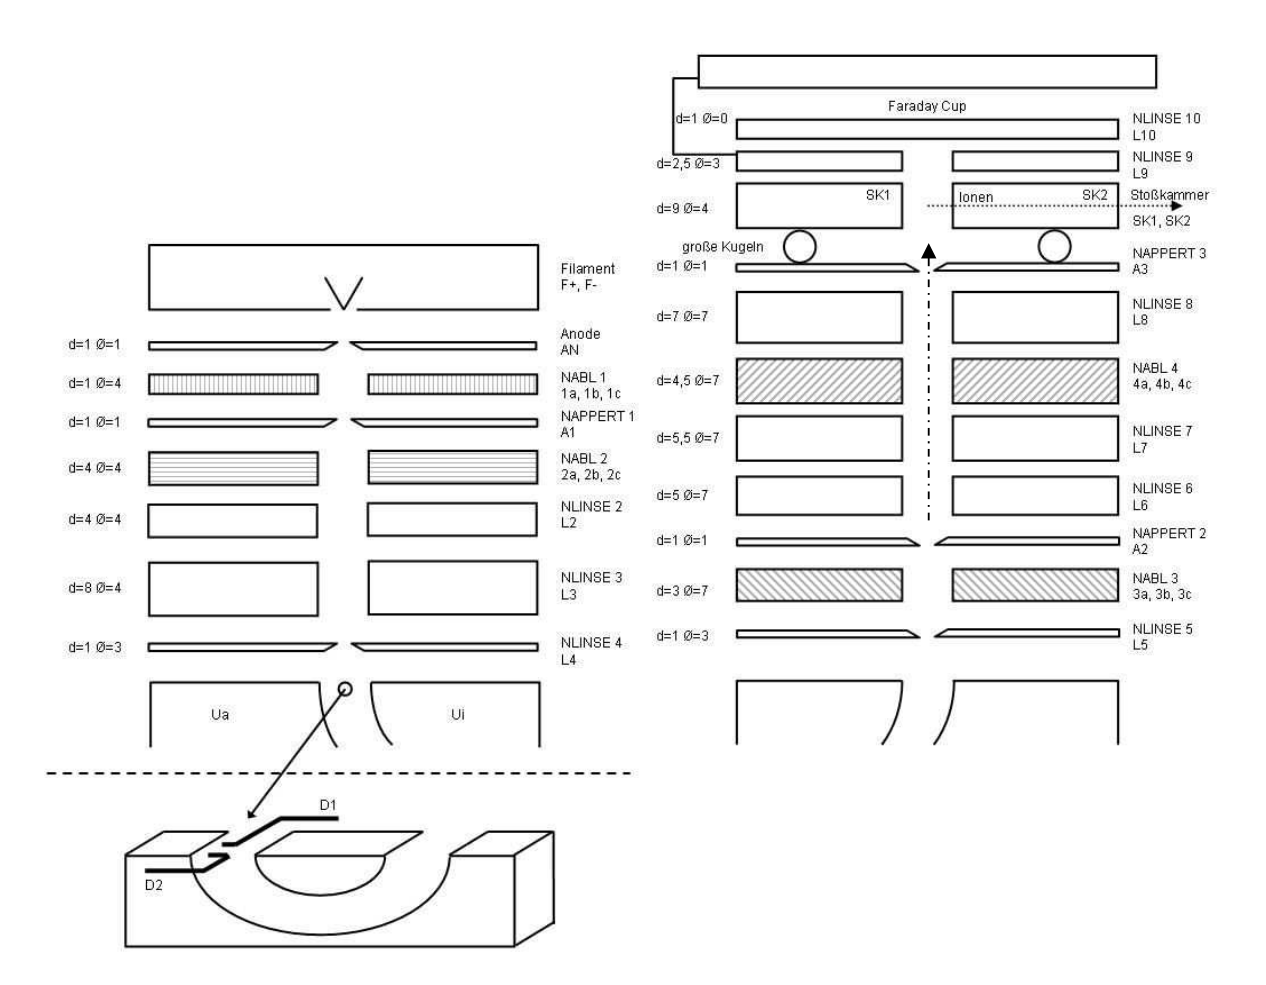
\includegraphics[width = 1 \textwidth]{setup.png}
	\caption{Layout of the used experimental setup, taken from \cite{script}. Electrons emitted by the filament are collected and guided by a set of electrostatic lenses into the hemispherical energy monochromator. Electrons with the right kinetic energy can pass and are guided via a second set of lenses into the collision chamber. }
	\label{setup}
\end{figure}

\subsection{Quadrupole mass filter}
The mass of the charged cluster is measured with a combination of a linear quadrupole mass filter and a channeltron detector. The channeltron can detect only the intensity of incoming ions, but not the $m/z$-ratio. Therefore a quadrupole filter is used select the ratio at which the intensity is of interest. In the experiment a program allows for automated scanning over a range of different masses. \\
Quadrupole filters are remarkably simple in terms of their structure. They consist of four metal rods of either cylindrical or hyperbolic shape that are placed in a square configuration \cite{ms_book}. The voltages applied to the rods have a AC and a DC component. Opposite rods are generally on the same voltage, while the rods next to a specified rod would have an opposite sign on the applied voltage. \\
If an ion is moving along in the direction of the rods it will be influenced by the electric field generated by the rods. Depending on the mass of the ion, the magnitude and frequency of the voltages and the radius of the configuration the ion will either pass through the quadrupole or collide with one of the rods and be filtered. \\
However, the resolution of a quadrupole cannot be indefinitely increased by tuning parameters, because ultimately the accuracy in the machining of the filter is the limiting factor. \\
Usually quadrupole filters operate at unit resolution, as is also the case in this experiment. Unit resolution means that the resolution inaccuracy is one unit mass (as in atomic mass unit) independent of the $m/z$-ratio at which the quadrupole is currently operating \cite{ms_book}.

\section{Analysis}
\subsection{Isotope population}\label{section:isotopes}
In the first part of the experiment, we took a look at the isotope distribution of neon clusters. We analyzed the mass spectrum from 25 up to around 130 mass charge ratio, this should be enough to look for cluster with size up to \ch{Ne6+}. In figure \ref{isotopespectrum} the full spectrum can be seen. The first peak appears at around 28, this is not due Neon clusters, but from residual air in the setup, in fact air is most molecular nitrogen \ch{N_2} which has a weight of $\approx 28$ u. The other peaks are at 40, 60, 80, 100 and 120 which are respectively \ch{Ne_2+}, \ch{Ne_3+}, \ch{Ne_4+}, \ch{Ne_5+}, and \ch{Ne_6+}. For the isotope population we can take at look at the peak around 40. We can see two peaks at 40.5 and 42.5. The neon abundance is 90.92\% for \ch{^{20}Ne}, 8.82\% for \ch{^{22}Ne}, and 0.26\% for \ch{^{21}Ne} \cite{script}, therefore we expect the first peak to correspond to a neon dimer of two \ch{^{20}Ne}, and the second peak corresponding to a neon dimer made of one \ch{^{20}Ne} and one \ch{^{22}Ne}. However the values do not match exactly the theoretical prediction of respectively 39.98 and 41.98 \cite{umc}. Apparently there is a systematic error of 0.5, maybe due to the calibration of our linear quadrupole mass spectrometer. To further investigate this problem we can take a look at the measurement around 60, here we can see three peaks at 60.5, 62.5 and 64.5, these are due to \ch{Ne3+} first made of three \ch{^{20}Ne}, and then made of two \ch{^{20}Ne} and one \ch{^{22}Ne}, and one \ch{^{20}Ne} and two \ch{^{22}Ne}. The calculated weight for this molecules are 59.98, 61.98, and 63.98, again we see the same pattern of systematic error. This is also confirmed for the two peaks around 80, we measured 80.6 and 82.6, which are for \ch{Ne4+} without isotopes and \ch{Ne4+} with one \ch{^{22}Ne} isotope, their theoretical values should be 79.97 and 81.97. For the cluster \ch{Ne5+} we have a peak at 100.7, another one at 102.6 and a small peak at 104.7, these are for \ch{Ne5+} without isotopes, \ch{Ne5+} with one \ch{^{22}Ne} isotope, and \ch{Ne5+} with two \ch{^{22}Ne} isotopes, their calculated values are 99.96, 101.96, and 103.96 respectively. For the last cluster \ch{Ne6+} we are able to see again three peaks at 120.7, 122.7, and 124.7 which correspond to \ch{Ne6+} without isotopes, \ch{Ne6+} with one \ch{^{22}Ne} isotope, and \ch{Ne6+} with two \ch{^{22}Ne} isotopes, their calculated values are 119.95, 121.95, and 123.95 respectively. In table \ref{isotopesresults} these results are summarized.  Furthermore we analyzed the height of the peaks to check whether is proportional to the relative abundance of the isotopes as we expect. For instance we took the peaks around 40, the proportion between the two peaks is 4.16:1 , which is not exactly as the expected 4.9:1 ratio, nevertheless is pretty close and confirm our hypothesis on the isotopes. For all the other peaks we have the same situation. The slightly disagreement could be explained in several ways, probably our source has a difference abundance, or it could be that the probability for \ch{^{20}Ne} and an isotopes to form a dimer, or a cluster are different due to different structure and binding energy.

\begin{figure}[H]
	\centering
	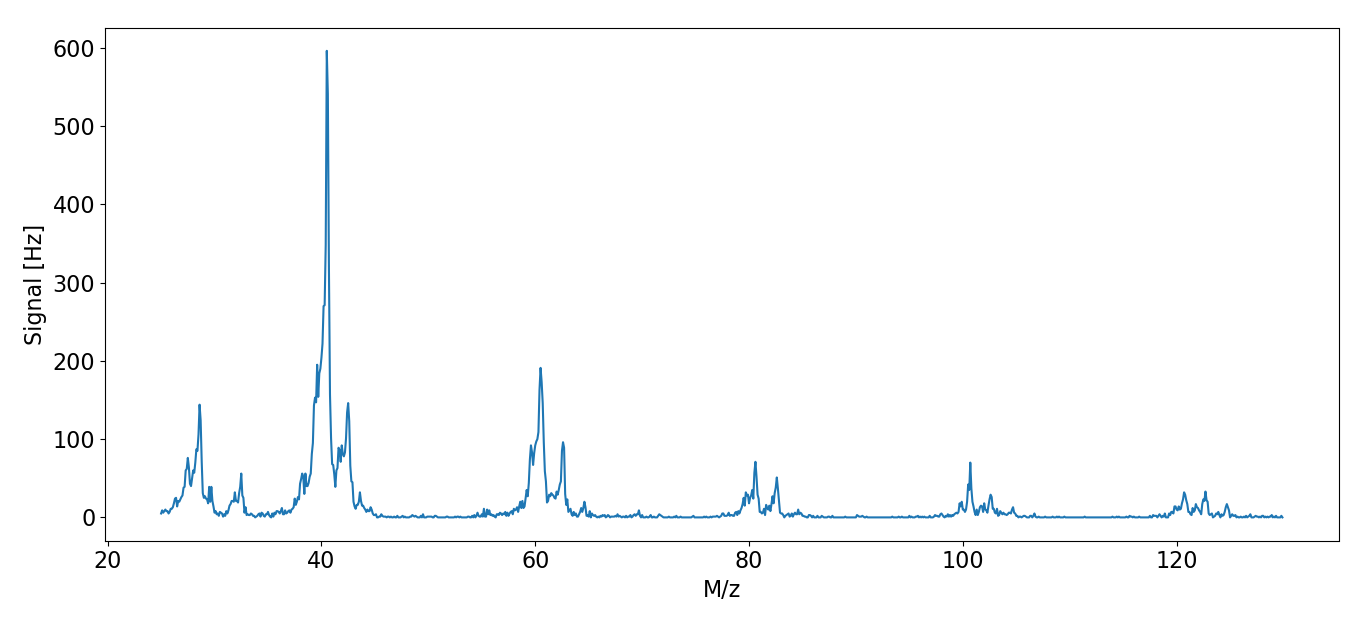
\includegraphics[width =\textwidth]{isotopespectrum}
	\caption{Mass spectrum of Neon clusters.}
	\label{isotopespectrum}
\end{figure}

\begin{table}[H]
\centering
\caption{Results for the Neon cluster spectrum. All theoretical calculations are made with the software \cite{umc}}\label{isotopesresults}
\begin{tabular}{ccc} \toprule
Measured peak (u/e) & Theoretical (u/e) & Isotope (charge +) \\ \midrule
40.5 & 39.98 & \ch{^{20}Ne2}\\
42.5 & 41.98 & \ch{(^{20}Ne)(^{22}Ne)}\\\midrule
60.5 & 59.98 & \ch{^{20}Ne3}\\
62.5 & 61.98 & \ch{(^{20}Ne)2(^{22}Ne)}\\
64.5 & 63.98 & \ch{(^{20}Ne)(^{22}Ne)2}\\\midrule
80.6& 79.97 & \ch{^{20}Ne4}\\
82.6& 81.97 & \ch{(^{20}Ne)3(^{22}Ne)}\\\midrule
100.7 & 99.96 & \ch{^{20}Ne5}\\
102.7 & 101.96 & \ch{(^{20}Ne)4(^{22}Ne)}\\
104.7 & 103.96 & \ch{(^{20}Ne)3(^{22}Ne)2}\\\midrule
120.7 & 119.95 & \ch{^{20}Ne6}\\
122.7 & 121.95 & \ch{(^{20}Ne)5(^{22}Ne)}\\
124.7 & 123.95 & \ch{(^{20}Ne)4(^{22}Ne)2}\\
\bottomrule
\end{tabular}
\end{table}


\subsection{Magic numbers}
In the next part of the experiment a measurement was conducted to look at magic numbers in the mass spectrum. Magic numbers are defined as a number of atoms where a cluster shows extraordinary behaviour, i.e. the there is a sudden change in the amplitude of a peak or the slope between the peaks changes suddenly. \\
We recorded the $m/Z$ ratio over a range of \SI{38}{} to \SI{330}{\atomicmassunit \per \elementarycharge}. Fig. \ref{fig_magic_peak} shows the result of the measurement. We can already see that number 13 and 14 do not follow the decreasing trend, but they present a plateau, furthermore at 15 we can notice a drop in intensity. To further investigate these magic numbers, we integrated the area beneath each peak and compared them to each other. This is shown in fig. \ref{fig_magic_simple}

\begin{figure}[H]
	\centering
	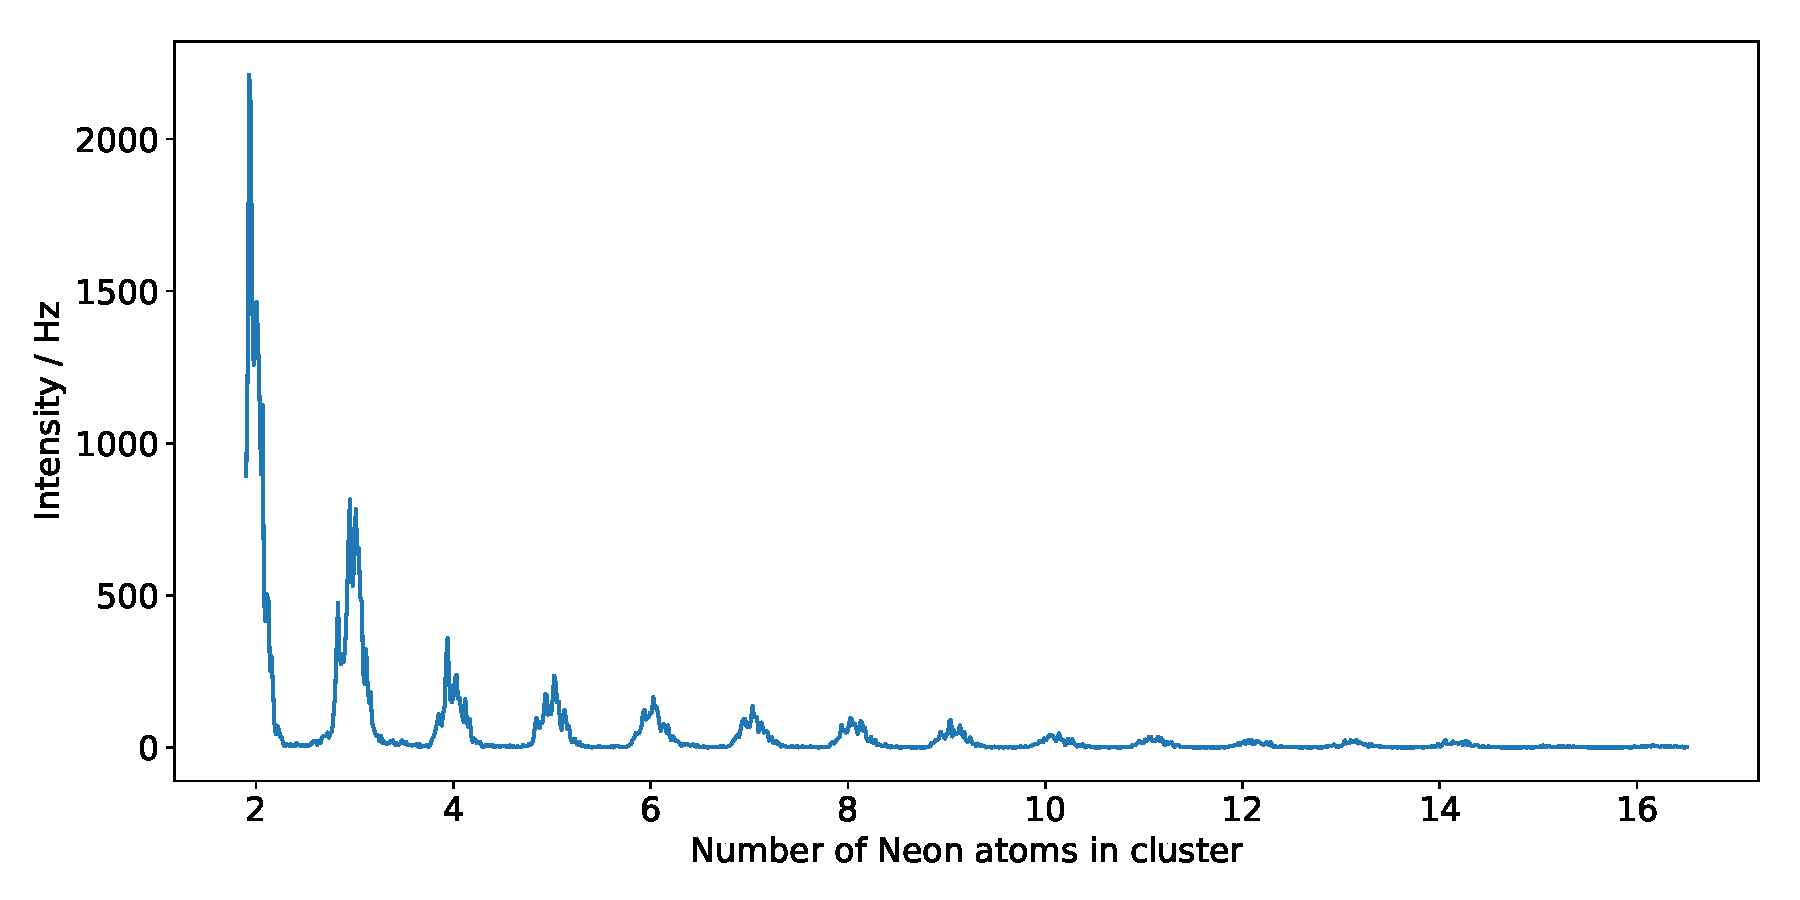
\includegraphics[width = 0.8 \textwidth]{magic_peaks}
	\caption{Depiction of the $m/z$ spectrum of \ch{Ne}-clusters from \SI{38}{} to \SI{330}{\atomicmassunit \per \elementarycharge} in logarithmic scale.}
	\label{fig_magic_peak}
\end{figure}

\begin{figure}[H]
  \centering{}
  \begin{subfigure}[t]{0.45 \textwidth}
    \centering
    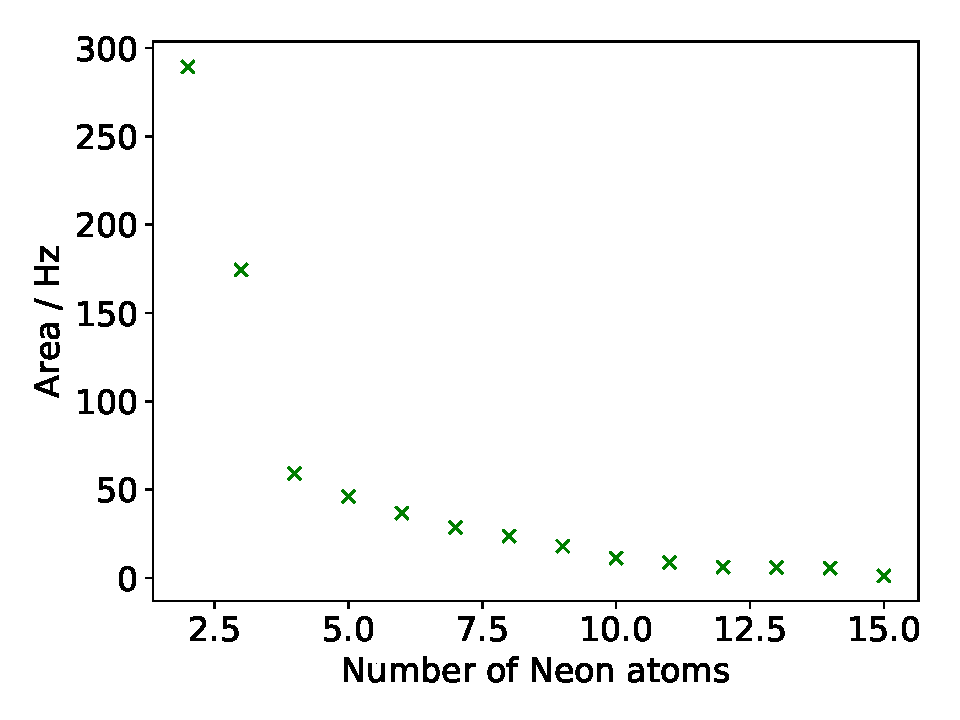
\includegraphics[height=6cm]{magic_area.pdf}
    \caption{Area of peaks.}
  \end{subfigure}
  ~
  \begin{subfigure}[t]{0.45 \textwidth}
    \centering
    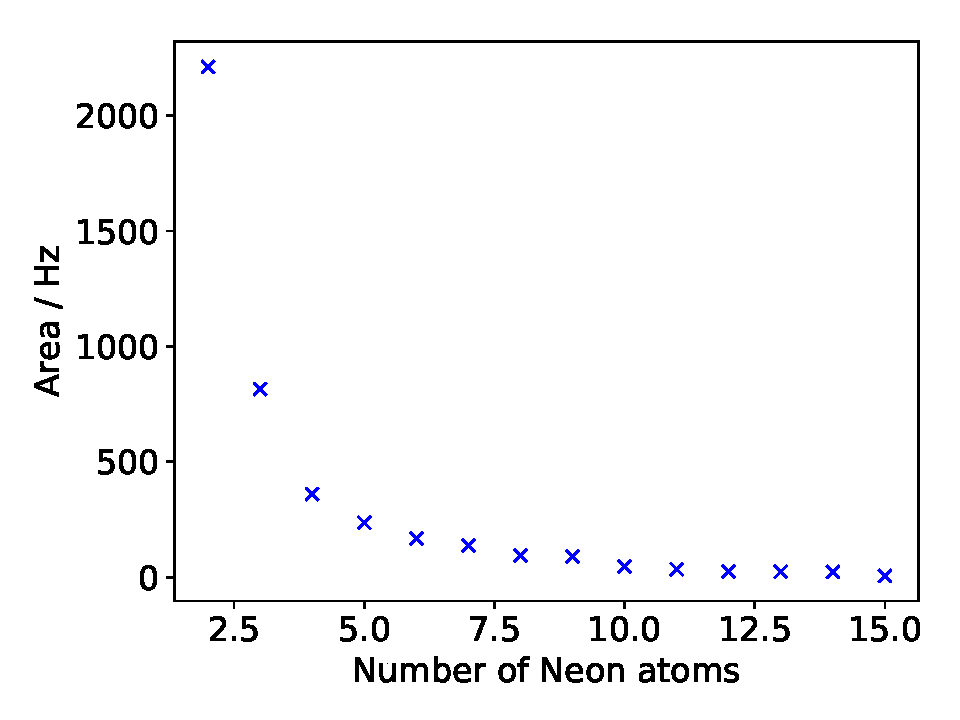
\includegraphics[height=6cm]{magic_height.pdf}
    \caption{Height of Peaks. }
  \end{subfigure}
  \caption{Plot of the area beneath the peaks and the height of the peaks in Fig. \ref{fig_magic_peak}}
  \label{fig_magic_simple}
\end{figure}
As can be seen in fig. \ref{fig_magic_simple} there is a plateau in the size of the clusters at 12, 13 and 14 atom clusters. In the other peaks there seems to be an exponential decline in clustersize. Since the peak at 12 seems to still be part of the declining line, we assume that only 13 and 14 are indeed magic numbers in the Neon cluster spectrum, although they are not really prominent peaks. \\
This seems to be in accordance with \cite{paper_scheier}, where it is stated that 13 is a magic number for clusters of icosahedral shape. They too reach the conclusion that \ch{Ne14+} qualifies as a magic number since it is followed by a comparably steep decline, which is also visible in fig. \ref{fig_magic_peak}.

\subsection{Appearance energy for Ne and Ne$_2$}
In the next section the appearance energy of the ionized monomer and dimer \ch{Ne+} and \ch{Ne2+} have to be measured. To measure the ionization energy of the Neon atom the mass selector was fixed to \SI{20.6}{\atomicmassunit}, and the energy of the electron beam was varied. The result for the monomer is shown in fig. \ref{fig_energy_monomer}.
\begin{figure}[H]
	\centering
	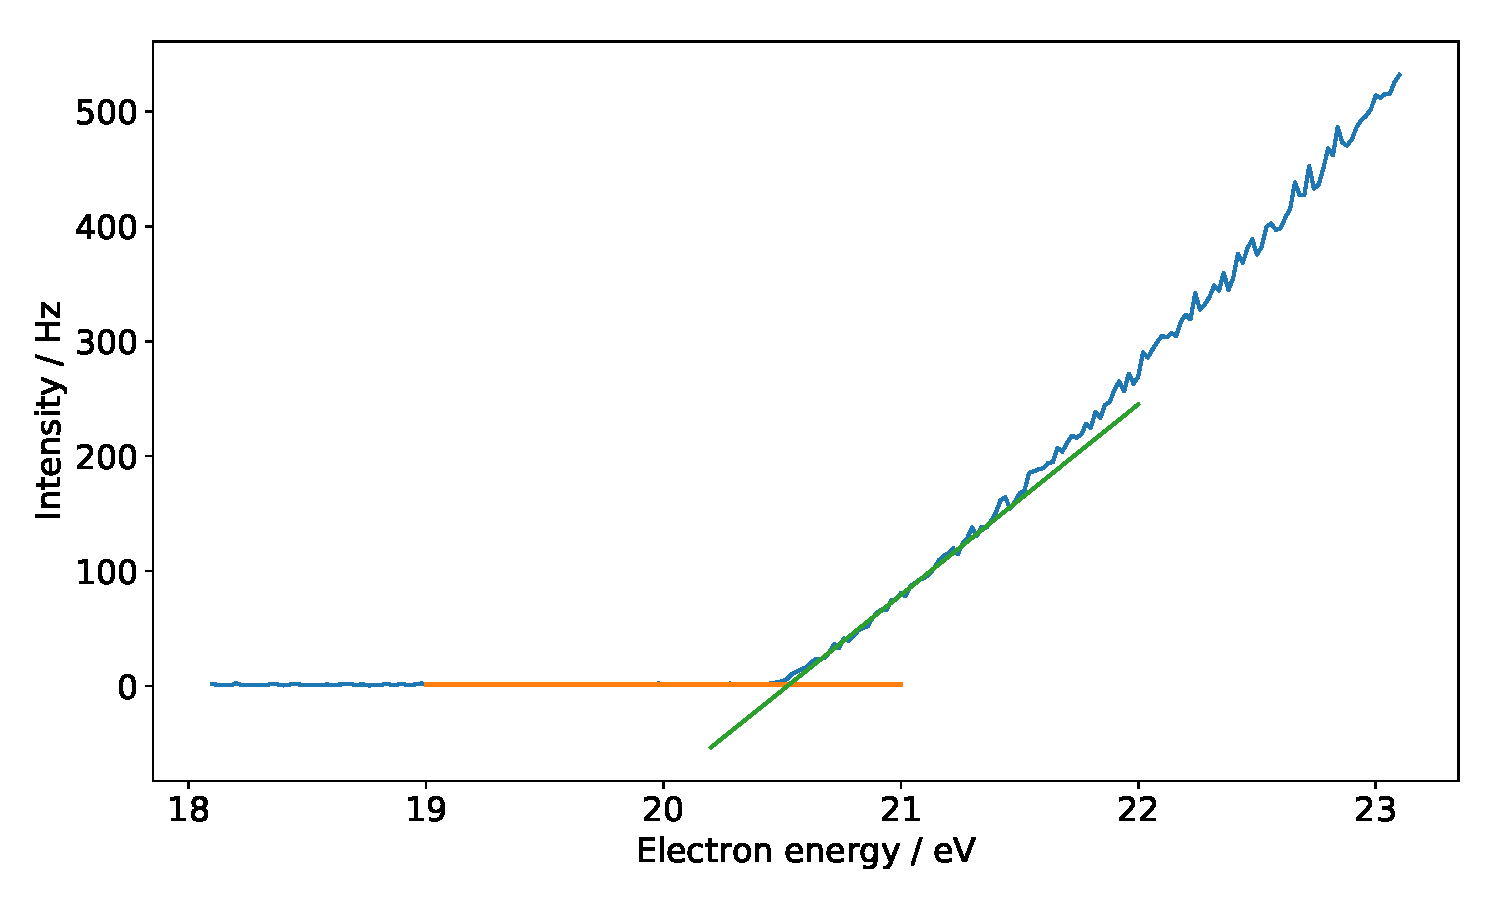
\includegraphics[width = 0.8 \textwidth]{energy_ne.pdf}
	\caption{Plot of the detected signal depending on the electron energy. The intersection of the lines is \SI{20}{\electronvolt}. The displacement of the constant function is $c=\SI{1.21(4)}{\hertz}$, while the parameters of the linear function are $a = \SI{165(3)}{\hertz \per \electronvolt}$ and $b = \SI{-3400(60)}{\hertz}$. This yields an intersection at \SI{20.53(1)}{\electronvolt}. }
	\label{fig_energy_monomer}
\end{figure}
The intersection of the constant and the linear function, which corresponds to the appearance energy, is found to be at \SI{20.53(1)}{\electronvolt} in fig. \ref{fig_energy_monomer}. According to \cite{neon_nist} the ionization energy is \SI{21.56454}{\electronvolt}. This result allows us to calibrate the energy axis for the appearance energy of the Neon dimer. \\
The calculation of the appearance energy of the dimer is done in an analogous way to the monomer. The mass selector is set to \SI{40.6}{\atomicmassunit}, then the energy range is again scanned in the range depicted in fig. \ref{fig_energy_dimer}.
\begin{figure}[H]
	\centering
	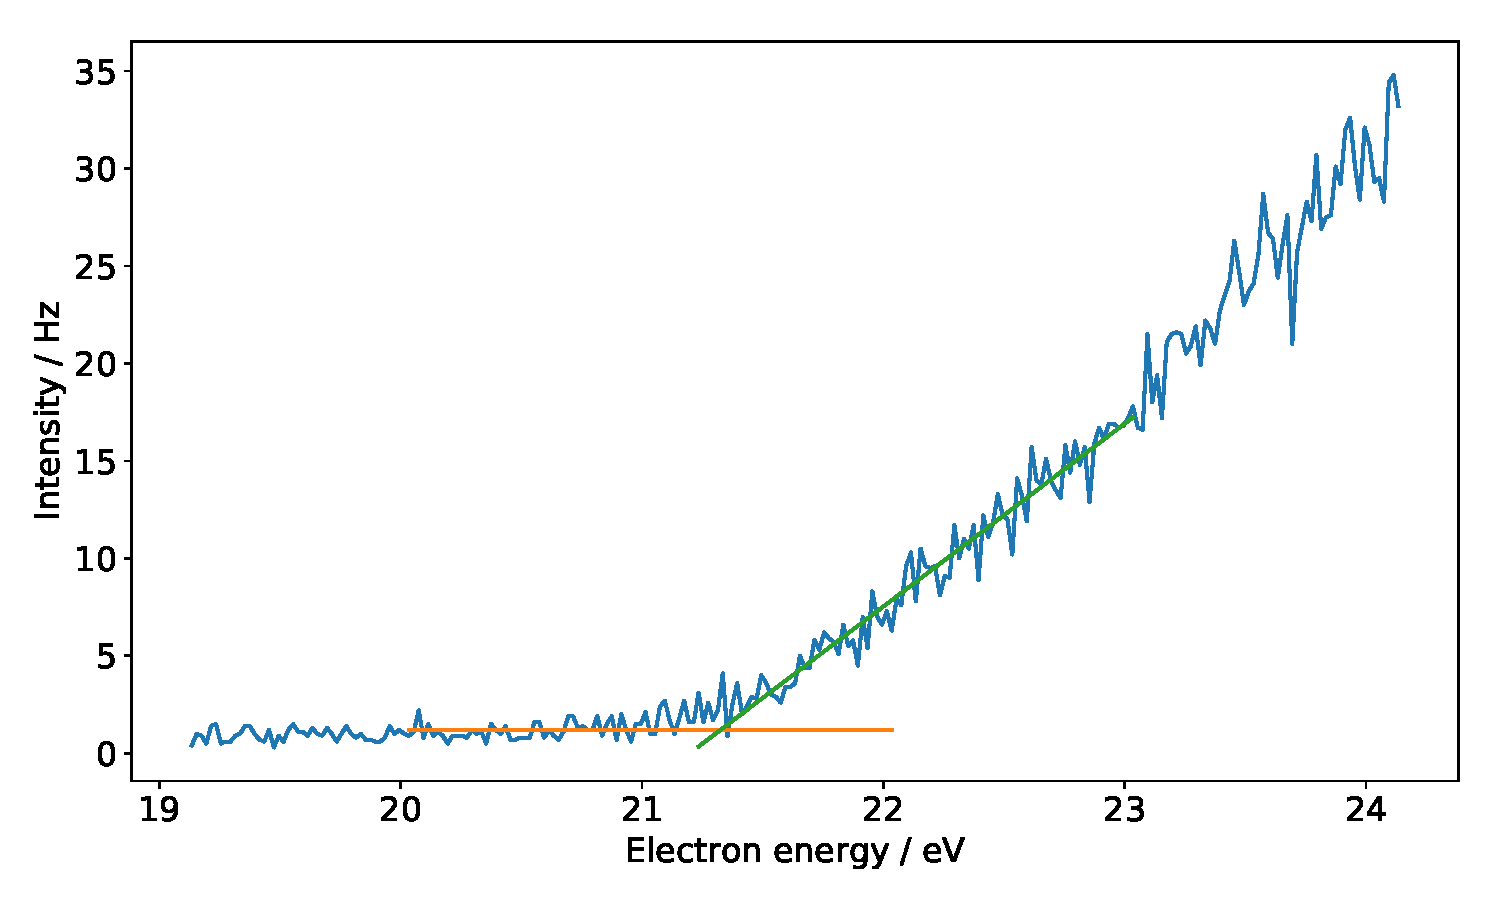
\includegraphics[width = 0.8 \textwidth]{energy_ne2.pdf}
	\caption{Depiction of the appearance energy for a Neon dimer. The energy axis was calibrated with the result of the monomer. The parameters determined through the fit were $c = \SI{1.18(5)}{\hertz}$ for the constant function, $a = \SI{9(1)}{\hertz \per \electronvolt}$ as the slope and $b = \SI{-200(20)}{\hertz}$ as the offset of the linear function. The intersection is found at \SI{21.32(7)}{\electronvolt}. Note that the intensity scale is different than in fig. \ref{fig_energy_monomer}. }
	\label{fig_energy_dimer}
\end{figure}
The intersection in fig. \ref{fig_energy_dimer} is located at \SI{21.32(7)}{\electronvolt}, which is in agreement with the previous value, since it has a larger error. Hence it takes approximately the same amount of energy to ionize a Neon atom or a Neon dimer. However, one will notice that even though fig. \ref{fig_energy_monomer} and \ref{fig_energy_dimer} look very similar the intensity scale is different by about a factor of $15$. \\
We assume this is simply because there is more monomers in the gas that is ionized than there are dimers. Looking at fig. \ref{isotopespectrum}, one can see that the intensity is increasing the smaller the cluster is. Therefore is plausible that the monomer is actually the most abundant component of the gas that is ionized.

\subsection{Pick-up}
In the last part of the experiment we studied the impact of a pickup gas in our cluster. We used simple air as pick up. The mass spectrum obtained is shown in figure \ref{pickup}. We can immediately notice two peaks on the left at 28.3 and 32.3, these are from the pickup gas, i.e. air which is manly \ch{N2} and \ch{O2} which are the peaks we see. In figure \ref{pickupzoom} a close up of the other peaks can be seen. Those peaks are one-two order of magnitude lower than the pickup peaks, but they present interesting features. First of all we recognize the same isotopes peaks of section \ref{section:isotopes}, but this time there are also more peaks in between them, which are clusters with the pickup gas nitrogen, oxygen, or both. In table \ref{pickupresults} we summarize all peaks, and our best guess of what they could be. We also observe the same systematic error of section \ref{section:isotopes}.
 From the results we can notice a couple of clusters with pick up gas, in two instances the neon cluster picked up the molecule \ch{N2}, in one case the pickup was of oxygen, and in another case the cluster picked up a \ch{NO} molecule.
 We also notice that in our experiment, clusters with a size $\geq 4$ neon atoms did not pick up any other element.

\begin{figure}[H]
	\centering
	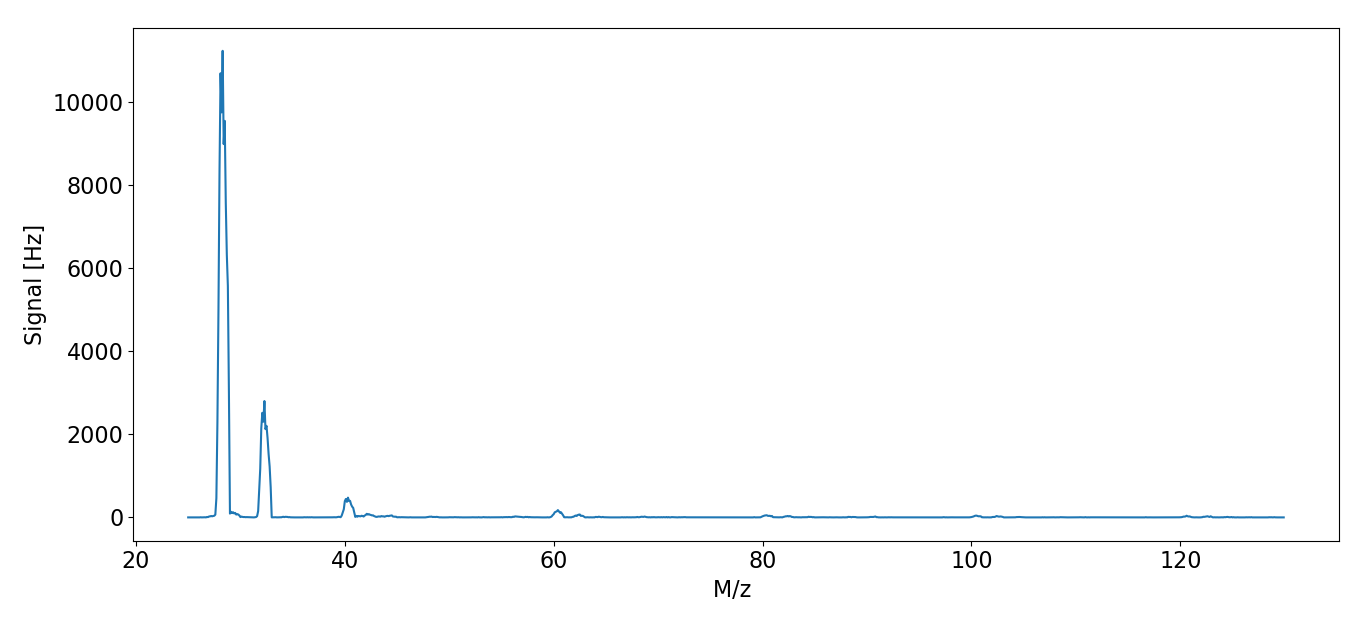
\includegraphics[width =\textwidth]{pickup}
	\caption{Mass spectrum of Neon clusters with air as pickup.}
	\label{pickup}
\end{figure}
\begin{figure}[H]
	\centering
	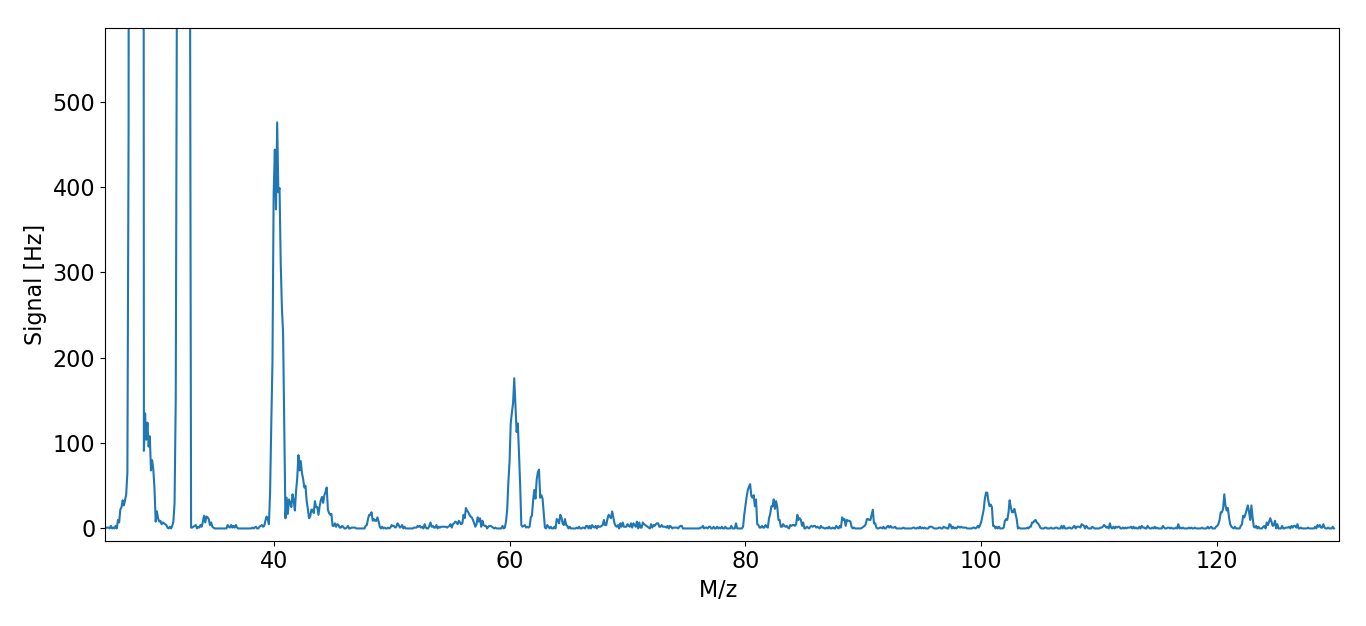
\includegraphics[width =\textwidth]{pickupzoom}
	\caption{Mass spectrum of Neon clusters with air as pickup.}
	\label{pickupzoom}
\end{figure}

\begin{table}[H]
\centering
\caption{Results for the Neon cluster spectrum with pickup. All theoretical calculations are made with the software \cite{umc}}\label{pickupresults}
\begin{tabular}{ccc} \toprule
Measured peak (u/e) & Theoretical (u/e) & Cluster composition (charge +) \\ \midrule
40.5 & 39.98 & \ch{^{20}Ne2}\\
42.5 & 41.98 & \ch{(^{20}Ne)(^{22}Ne)}\\
44.5 & 44.00 &\ch{N2O}\\
56.5 & 55.98 & \ch{Ne2O}\\ \midrule
60.5 & 59.98 & \ch{^{20}Ne3}\\
62.5 & 61.98 & \ch{(^{20}Ne)2(^{22}Ne)}\\
64.5 & 63.98 & \ch{(^{20}Ne)(^{22}Ne)2}\\
68.5 & 67.99 & \ch{Ne2N2}\\\midrule
80.4& 79.97 & \ch{^{20}Ne4}\\
82.4& 81.97 & \ch{(^{20}Ne)3(^{22}Ne)}\\
84.4 & 83.97 & \ch{(^{20}Ne)2(^{22}Ne)2}\\
88.5 & 87.98 & \ch{N2Ne3}\\
90.5 & 89.97 & \ch{Ne3NO}\\\midrule
100.5 & 99.96 & \ch{^{20}Ne5}\\
102.5 & 101.96 & \ch{(^{20}Ne)4(^{22}Ne)}\\
104.7 & 103.96 & \ch{(^{20}Ne)3(^{22}Ne)2}\\\midrule
120.6 & 119.95 & \ch{^{20}Ne6}\\
122.6 & 121.95 & \ch{(^{20}Ne)5(^{22}Ne)}\\
124.6 & 123.95 & \ch{(^{20}Ne)4(^{22}Ne)2}\\
\bottomrule
\end{tabular}
\end{table}

\section{Conclusion}

\begin{thebibliography}{99}

\bibitem{script}
\textsc{Stephan Denifl}, \textit{FP3‐Praktikumsversuch – Edelgascluster/Rare gas clusters (SS 2018)}, 2018

\bibitem{bergmann}
\textsc{Bergmann-Schäfer}, \textit{Gase, Nanosysteme, Flüssigkeiten}, \textit{Band 5} (de Gruyter, 2005)

\bibitem{ms_book}
\textsc{Jürgen H. Gross}, \textit{Mass Spectrometry}, Springer, 2nd Edition, 2011

\bibitem{neon_nist}
\textsc{Nist}, \textit{Basic Atomic Spectroscopic Data - Neon (Ne)}, \url{https://www.physics.nist.gov/PhysRefData/Handbook/Tables/neontable1.htm}

\bibitem{paper_scheier}
\textsc{T.D. Märk, P. Scheier}, \textit{PRODUCTION AND STABILITY OF NEON CLUSTER IONS UP TO } \ch{Ne90+}, Chemical Physics Letters Vol. 137, Number 3, 12 June 1987

\bibitem{umc}
\textsc{Matthias Letzel}, \textit{Universal Mass Calculator - Student Edition}, Universität Münster, \url{https://www.uni-muenster.de/Chemie.oc/ms/downloads.html}
\end{thebibliography}

\end{document}
